% ============================================================
%  Reporte del modelo fisico - Laboratorio 4
%  Compilar con: pdflatex reporte_modelo.tex  (dos veces)
% ============================================================
\documentclass[11pt,a4paper]{article}

\usepackage[utf8]{inputenc}
\usepackage[T1]{fontenc}
\usepackage[spanish,es-noquoting]{babel}
\usepackage{lmodern}
\usepackage[margin=2.2cm,top=1.9cm,bottom=1.9cm]{geometry}
\usepackage{xcolor}
\usepackage{enumitem}
\usepackage{listings}
\usepackage{titlesec}
\usepackage{float}
\usepackage{graphicx}
\usepackage{tikz}
\usetikzlibrary{shapes.geometric,arrows.meta,positioning,calc}
\usepackage[colorlinks=true,urlcolor=blue!55!black]{hyperref}

\setlist[itemize]{topsep=2pt,itemsep=1.5pt,parsep=0pt,leftmargin=1.2em}
\setlist[enumerate]{topsep=2pt,itemsep=1.5pt,parsep=0pt,leftmargin=1.4em}
\setlength{\parskip}{3pt}
\pagestyle{empty}

\titleformat{\section}{\normalsize\bfseries}{}{0pt}{}
\titlespacing*{\section}{0pt}{9pt}{2pt}

% --- estilo de los listados de código ---
\lstset{
  language=C,
  basicstyle=\ttfamily\scriptsize,
  commentstyle=\color{black!55}\itshape,
  keywordstyle=\bfseries,
  showstringspaces=false,
  tabsize=2,
  frame=leftline,
  framerule=0.6pt,
  rulecolor=\color{black!40},
  xleftmargin=8pt,
  aboveskip=4pt,
  belowskip=2pt,
  literate={á}{{\'a}}1 {é}{{\'e}}1 {í}{{\'i}}1 {ó}{{\'o}}1 {ú}{{\'u}}1
           {ñ}{{\~n}}1 {¿}{{?`}}1 {→}{{$\to$}}1
}

% --- estilo del diagrama ---
\tikzset{
  paso/.style={rectangle, rounded corners=3pt, draw=black!60, fill=blue!6,
               text width=10.2cm, align=left, inner sep=3pt, font=\footnotesize},
  decision/.style={diamond, aspect=3.5, draw=black!60, fill=orange!12,
                   align=center, inner sep=0pt, font=\footnotesize},
  mecanica/.style={rectangle, rounded corners=3pt, draw=black!60, fill=red!8,
                   text width=3.8cm, align=left, inner sep=3pt, font=\footnotesize},
  flecha/.style={-{Stealth[length=2.2mm]}, thick, black!70}
}

\begin{document}
\begin{center}
{\large\bfseries Laboratorio 4: modelo físico del balancín}\\[2pt]
Ensayos del 24 de noviembre de 2026
\end{center}

\section{Qué busqué}
Quería un modelo de la maqueta para elegir las ganancias del PID, sin agregados en el código (sin empujón y sin banda muerta).

\section{Cómo medí}
Primero hice un escalón en lazo cerrado (Kp 3, Ki 0, Kd 0,8) y lo analicé con el script de MATLAB. Dio K = 0,45~cm/s² por grado de servo. El método de Chen no se pudo usar porque el sobrepico pasó el 100\,\%.

Después apagué el PID, dejé el servo en un ángulo fijo y grabé cómo rodaba la pelota cada 50~ms. Hice 18 corridas, con distintos ángulos y puntos de partida.

\begin{figure}[H]\centering
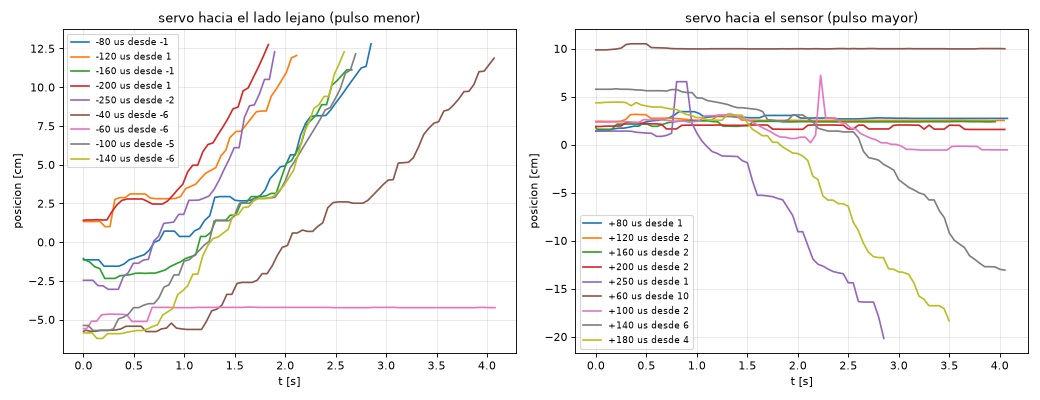
\includegraphics[width=0.95\textwidth]{lazo_abierto.png}
\caption{Corridas en lazo abierto. Los valores son microsegundos respecto de 1525.}
\end{figure}

Vi dos cosas. La pelota avanza a velocidad casi constante, como si un roce la frenara. Y hacia el lado lejano llegó a arrancar con 40~µs de diferencia, pero hacia el sensor en general necesitó más de 100. Eso sugiere que 1525~µs no es la horizontal.

\section{Cómo saqué el modelo}
Derivar dos veces la posición no sirvió, porque el ruido del sensor tapa la aceleración. Entonces ajusté por simulación: tomo tramos de 1~s, le doy al modelo el ángulo del servo y comparo la posición simulada con la medida. Sumé registros en lazo cerrado y validé con ensayos enteros que no usé en el ajuste.
\[ a = K(\theta-\theta_0) - b\,v \]

\begin{center}\small
\begin{tabular}{lcccc}
\hline
Modelo & $K$ & $\theta_0$ & $b$ & Error en 1 s\\ \hline
Suponer la pelota quieta & & & & 2,01 cm\\
M1: sin roce & 0,78 & $-5{,}3^\circ$ & 0 & 2,73 cm\\
M2: con roce viscoso & 1,27 & $-5{,}7^\circ$ & 5,2 & 1,82 cm\\
M3: M2 más roce estático & 1,75 & $-3{,}8^\circ$ & 7,1 & 1,80 cm\\ \hline
\end{tabular}
\end{center}

El roce viscoso mejora el modelo y el estático casi no agrega nada. Igual, el modelo predice poco: gana apenas contra suponer la pelota quieta, y $K$ y $b$ cambian bastante según los datos. Lo más repetido es que $\theta_0$ da negativo, lo que pone la horizontal entre 1567 y 1588~µs. También noté que la pelota suele frenarse cerca de +2 o +3~cm. Puede ser un bache, pero no lo confirmé.

\section{Qué valores probé en la maqueta}
\begin{center}\small
\begin{tabular}{lp{9.6cm}}
\hline
Kp / Ki / Kd & Resultado\\ \hline
2,5 / 0,3 / 0,8 & Con horizontal 1315 se trabó. Con 1525 quedó cerca del centro\\
1,5 / 0 / 0,8 & La pelota no se movió\\
3 / 0 / 0,8 & Escalón de 8 cm: llegó hasta 15 cm\\
3 / 0 / 1,5 & Menos sobrepico\\
3 / 0,2 / 1,5 & Servo a 60 grados/s: 87\,\% del tiempo dentro de 2 cm (con banda de 1 cm)\\
3 / 0,2 / 0,8 & Servo a 150 grados/s: oscila mucho\\
3 / 0,4 / 1,5 & Se traba y al soltarse se pasa\\
3 / 0,2 / 1,5 & Con empujón de 12 grados: oscila\\
2 / 0,1 / 1,5 & Con empujón: quieta queda casi siempre dentro de 1 cm, pero tras los escalones solo entre el 7 y el 50\,\% del tiempo\\
2 / 0,1 / 2,5 & Con empujón: oscila más\\ \hline
\end{tabular}
\end{center}
El empujón y la banda los saqué, porque quería un PID puro.

\section{Qué opciones salieron del modelo}
Simulé el lazo copiando el firmware. Busqué entre 150 combinaciones con un primer ajuste de M2 y después revisé las principales con los modelos de la tabla. El porcentaje es el tiempo dentro de 1~cm al final de cada tramo:
\begin{center}\small
\begin{tabular}{lcccc}
\hline
Opción & Horizontal & Kp / Ki / Kd & Con M2 & Con M3\\ \hline
A & 1592 µs & 4 / 0,1 / 0,5 & 100\,\% & 100\,\%\\
B & 1525 µs & 4 / 0,8 / 0,5 & 100\,\% & 62\,\%\\
Anterior & 1525 µs & 3 / 0,2 / 1,5 & 74\,\% & 51\,\%\\ \hline
\end{tabular}
\end{center}

\section{Conclusión}
Elijo la opción A porque anda bien con los dos modelos con roce. Es un resultado de simulación y todavía no la probé en la maqueta. Los riesgos son que el modelo predice poco, que los 1592~µs salieron del primer ajuste y que Kd 0,5 es el valor más chico de la búsqueda, bastante menor al que venía usando. El próximo paso es repetir los escalones con la opción A y comparar.

\end{document}
